\documentclass[tikz]{standalone}
\usetikzlibrary{automata,positioning}
\begin{document}
  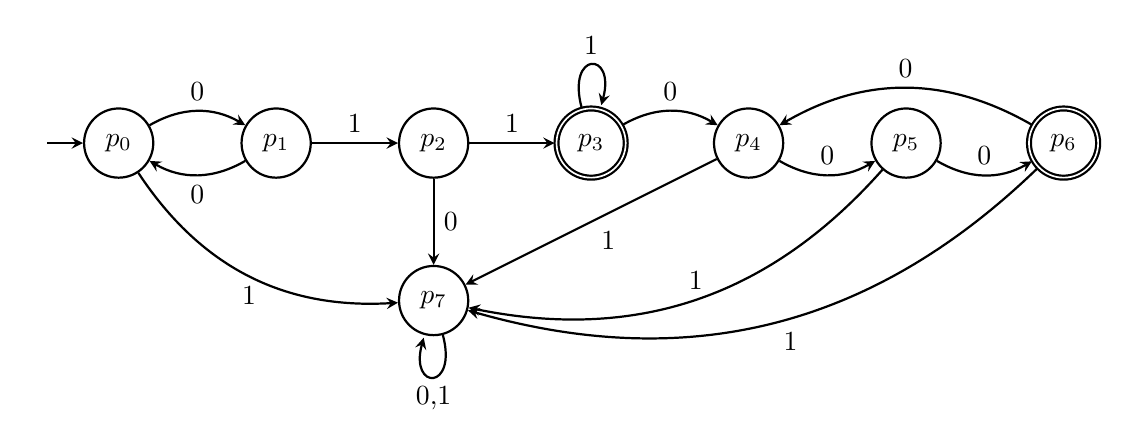
\begin{tikzpicture}[>=stealth,node distance=20mm,on grid,auto, thick, initial text=]
    \node[state,initial] (p0) {$p_0$};
    \node[state] (p1) [right=of p0] {$p_1$};
    \node[state] (p2) [right=of p1] {$p_2$};
    \node[state,accepting] (p3) [right=of p2] {$p_3$};
    \node[state] (p4) [right=of p3] {$p_4$};
    \node[state] (p5) [right=of p4] {$p_5$};
    \node[state, accepting] (p6) [right=of p5] {$p_6$}; 
    \node[state] (p7) [below=of p2] {$p_7$};
    
    \path[->]
    (p0) edge [bend left] node {0} (p1)
    (p0) edge [bend right] node [below] {1} (p7)
    (p1) edge [bend left] node {0} (p0)
    (p1) edge node {1} (p2)
    (p2) edge node {1} (p3)
    (p2) edge node {0} (p7)
    (p3) edge [loop above] node {1} (p3)
    (p3) edge [bend left] node {0} (p4)
    (p4) edge [bend right] node {0} (p5)
    (p4) edge node {1} (p7)
    (p5) edge [bend right] node {0} (p6)
    (p5) edge [bend left] node [above] {1} (p7)
    (p6) edge [bend right] node [above] {0} (p4)
    (p6) edge [bend left] node {1} (p7)
    (p7) edge [loop below] node {0,1} (p7);  
  \end{tikzpicture}

\end{document}